\chapter{Histograms and Beyond:  Nonparametric Density Estimation}
\label{chap:nonpardens}

Here we will be concerned with estimating density functions in settings
in which we do not assume our distribution belongs to some parametric
model.

Why is this important?  Actually, you've been seeing density estimates
for years---except that they've been called {\it histograms}---and
hopefully you are convinced that histograms are indeed useful tools for
data visualization.  Simply reporting the (estimated) mean and variance
of a distribution may not capture the nuances.

Moreover, density estimates can be used in {\it clasification} problems,
in which we are trying to get the class of something, based on other
variables.  In a medical context, for instance, we may be trying
predict whether a patient will develop a certain disease, knowing her
current test results, family history and so on.  We'll cover such
problems in Chapter \ref{chap:class}, but for now what is important to
know is that the clasification problem can be expressed in terms of
ratios of densities.

But guess what!  Histograms are actually density estimates, as we will
see.  And we can do better than histograms, with more sophisticated
density estimates.

% \subsection{The Empirical cdf}
% \label{ecdf}
% 
% Recall that $F_X$, the cdf of $X$, is defined as
% 
% \begin{equation}
% F_X(t) = P(X \leq t), ~ -\infty < t < \infty
% \end{equation}
% 
% Define its sample analog, called the {\bf empirical distribution
% function}, by
% 
% \begin{equation}
% \widehat{F}_X(t) = \frac{\# ~of~ X_i ~in~(-\infty,t)}{n}
% \end{equation}
% 
% In other words, $F_X(t)$ is the proportion of X that are below t in the
% population, and $\widehat{F}_X(t)$ is the value of that proportion in our
% sample.  $\widehat{F}_X(t)$ estimates $F_X(t)$ for each t.
% 
% Graphically, $\widehat{F}_X$ is a step function, with jumps at the values of
% the $X_i$.  Specifically, let $Y_j$, j = 1,...,n denote the sorted
% version of the $X_I$.\footnote{A common notation for this is
% $Y_j = X_{(j)}$, meaning that $Y_j$ is the $j^{th}$ smallest of the
% $X_i$.  These are called the {\bf order statistics} of our sample.}
% Then
% 
% \begin{equation}
% \widehat{F}_X(t) = 
% \begin{cases}
% 0, & \text{for $t < Y_1$} \\
% \frac{j}{n}, & \text{for $Y_j \leq t < Y_{j+1}$} \\
% 1, & \text{for $t > Y_n$} \\
% \end{cases} 
% \end{equation}
% 
% Here is a simple example.  Say n = 4 and our data are 4.8, 1.2, 2.2 and
% 6.1.  We can plot the empirical cdf by calling R's {\bf ecdf()}
% function:
% 
% \begin{Verbatim}[fontsize=\relsize{-2}]
% > plot(ecdf(x))
% \end{Verbatim}
% 
% Here is the graph:
% 
% 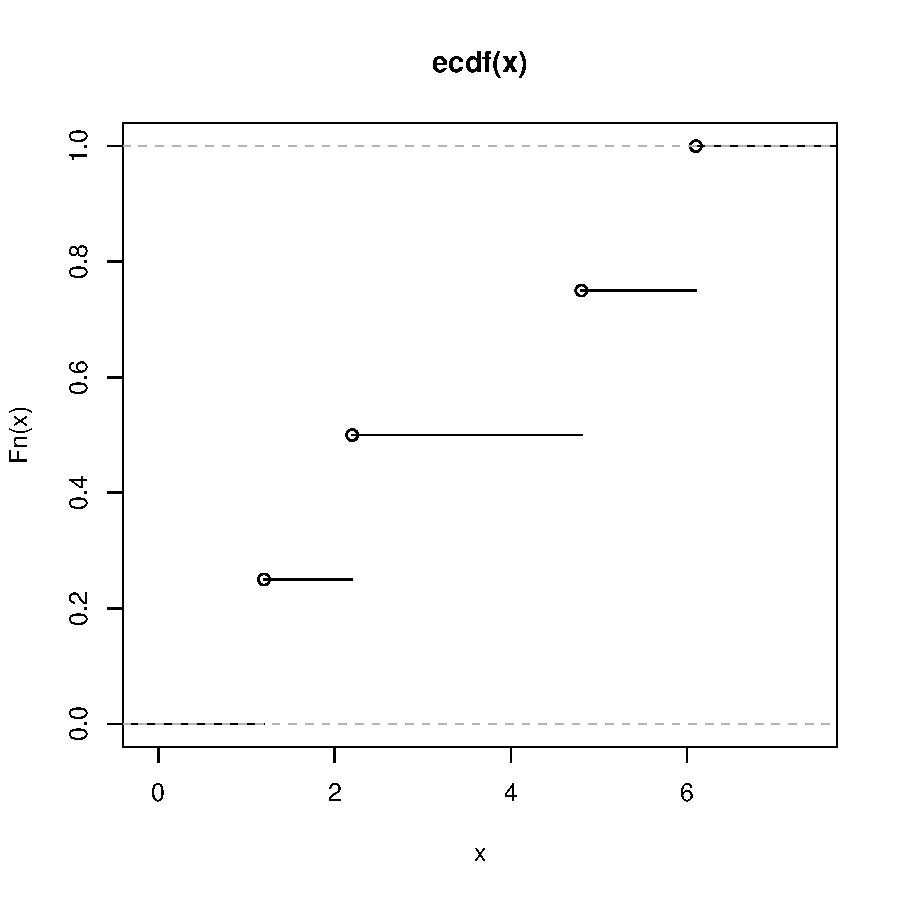
\includegraphics[width=3.0in]{EmpCDF.pdf} 
% 
% Consider the Bus Paradox example again.  Recall that $W$ denoted the
% time until the next bus arrives.  This is called the {\bf forward
% recurrence time}.  The {\bf backward recurrence time} is the time since
% the last bus was here, which we will denote by $R$.  
% 
% Suppose we are interested in estimating the density of $R$, $f_R()$,
% based on the sample data $R_1,...,R_n$ that we gather in our simulation
% in Section \ref{bus}, where n = 1000.  How can we do
% this?\footnote{Actually, one can prove that R has an exponential
% distribution.  However, here we'll pretend we don't know that.}
% 
% We could, of course, assume that $f_R$ is a member of some parametric
% family of distributions, say the two-parameter gamma family.  We would
% then estimate those two parameters as in Section \ref{genest}, and
% possibly check our assumption using goodness-of-fit procedures,
% discussed in our unit on modeling, Chapter \ref{chap:mod}.  On the other
% hand, we may wish to estimate $f_R$ without making any parametric
% assumptions.  In fact, one reason we may wish to do so is to visualize
% the data in order to search for a suitable parametric model.
% 
% If we do not assume any parametric model, we have in essence change our
% problem from estimating a finite number of parameters to an
% infinite-parameter problem; the ``parameters'' are the values of $f_X(t)$ 
% for all the different values of t.  Of course, we probably are willing
% to assume {\it some} structure on $f_R$, such as continuity, but then we
% still would have an infinite-parameter problem.
% 
% We call such estimation {\bf nonparametric}, meaning that we don't use a
% parametric model.  However, you can see that it is really 
% infinite-parametric estimation.
% 
% Again discussed in our unit on modeling, Chapter \ref{chap:mod}, the more
% complex the model, the higher the variance of its estimator.  {\bf So,
% nonparametric estimators will have higher variance than parametric
% ones.}  The nonparametric estimators will also generally have smaller
% bias, of course.

\section{Example:  Baseball Player Data}

In the data in Section \ref{baseball0}, suppose we are looking at
player's weights $W$, and we are interested in $f_W(182)$, the
population density for weights, evaluated at 182.  Our 
data is considered to be a sample from the populatin of all major league
players, past, present and future,\footnote{Recall Section
\ref{observational}.} and we will use this data to develop an estimate,

\begin{equation}
\widehat{f}_W(142)
\end{equation}

for the population quantity

\begin{equation}
f_W(182)
\end{equation}

But how can we do this?

\section{Basic Ideas in Density Estimation}

Suppose we have a random sample $R_1,...,R_n$ from a distribution $F_R$.
How can we estimate $f_R$ from the $R_i$?

Recall from the first day of your calculus course that for a function
$g()$

\begin{equation}
g'(x) = \lim_{h \rightarrow 0} \frac{g(x+h) - g(x)}{h}
\end{equation}

and thus for small $h$,

\begin{equation}
g'(x) \approx \frac{g(x+h) - g(x)}{h}
\end{equation}

Now take $g()$ to be $F_R()$ for our random variable $R$ above, so that 

\begin{equation}
f_R(t) \approx \frac{F_R(t+h) - F_R(t)}{h}
\end{equation}

We can alter this a little:  Instead of looking at the interval
$(t,t+h)$, we can use $(t-h,t+h)$:

\begin{equation}
f_R(t) \approx \frac{F_R(t+h) - F_R(t-h)}{2h}
\end{equation}

That means that

\begin{eqnarray}
\label{diffquot}
f_R(t) &\approx& \frac{F_R(t+h) - F_R(t-h)}{2h} \\
&=& \frac{P(R \leq t+h) - P(R \leq t-h)}{2h} \\
&=& \frac{P(t-h < R \leq t+h)}{2h}
\end{eqnarray}

if h is small.  We can then form an estimate $\widehat{f}_R(t)$ by plugging
in sample analogs in the right-hand side of (\ref{diffquot}):

\begin{eqnarray}
\widehat{f}_R(t) &=& \frac{\#(t-h,t+h)/n}{2h} \\ 
&=& \frac{\#(t-h,t+h)}{2hn}  
\label{prehisto}
\end{eqnarray}

where the notation $\#(a,b)$ means the number of $R_i$ in the interval
(a,b).

There is an important issue of how to choose the value of h here, but
let's postpone that for now.  For the moment, let's take 

\begin{equation}
\label{h100}
h = \frac{\max_i R_i - \min_iR_i}{100}
\end{equation}

i.e. take h to be 0.01 of the range of our data.

At this point, we'd then compute (\ref{prehisto}) at lots of different
points t.  Although it would seem that theoretically we must compute
(\ref{prehisto}) at infinitely many such points, the graph of the
function is actually a step function.  Imagine t moving to the right,
starting at $\min_iR_i$.  The interval $(t-h,t+h)$ moves along with it.
Whenever the interval moves enough to the right to either pick up a new
$R_i$ or lose one that it had had,  (\ref{prehisto}) will change value,
but not at any other time.  So, we only need to evaluate the function at
about $2n$ values of t.

\section{Histograms} 

If for some reason we really want to save on computation, let's again
say that we first break the interval $(\min_iR_i, \max_iR_i)$ into 100
subintervals of size h given by (\ref{h100}).  We then compute
(\ref{prehisto}) only at the midpoints of those intervals, and assume
that the graph of $\widehat{f}_R(t)$ is approximately constant within
each subinterval (true for small h).  Do you know what we get from that?
A histogram!  Yes, a histogram is a form of density estimation.
(Usually a histogram merely displays counts.  We do so here too, but we
have scaled things so that the total area under the curve is 1, a
property of densities.)

% Let's see how this works with our Bus Paradox simulation from Section
% \ref{ciintro}.  We'll use R's {\bf hist()} to draw a histogram.  First,
% here's our simulation code:
% 
% \begin{Verbatim}[fontsize=\relsize{-2},numbers=left]
% doexpt <- function(opt) {
%    lastarrival <- 0.0
%    while (TRUE) {
%       newlastarrival = lastarrival + rexp(1,0.1)
%       if (newlastarrival > opt)
%          return(opt-lastarrival)
%       else lastarrival <- newlastarrival
%    }
% }
% 
% observationpt <- 240
% nreps <- 10000
% waits <- vector(length=nreps)
% for (rep in 1:nreps) waits[rep] <- doexpt(observationpt)
% hist(waits)
% \end{Verbatim}
% 
% Note that I used the default number of intervals, 20.  Here is the
% result:
% 
% 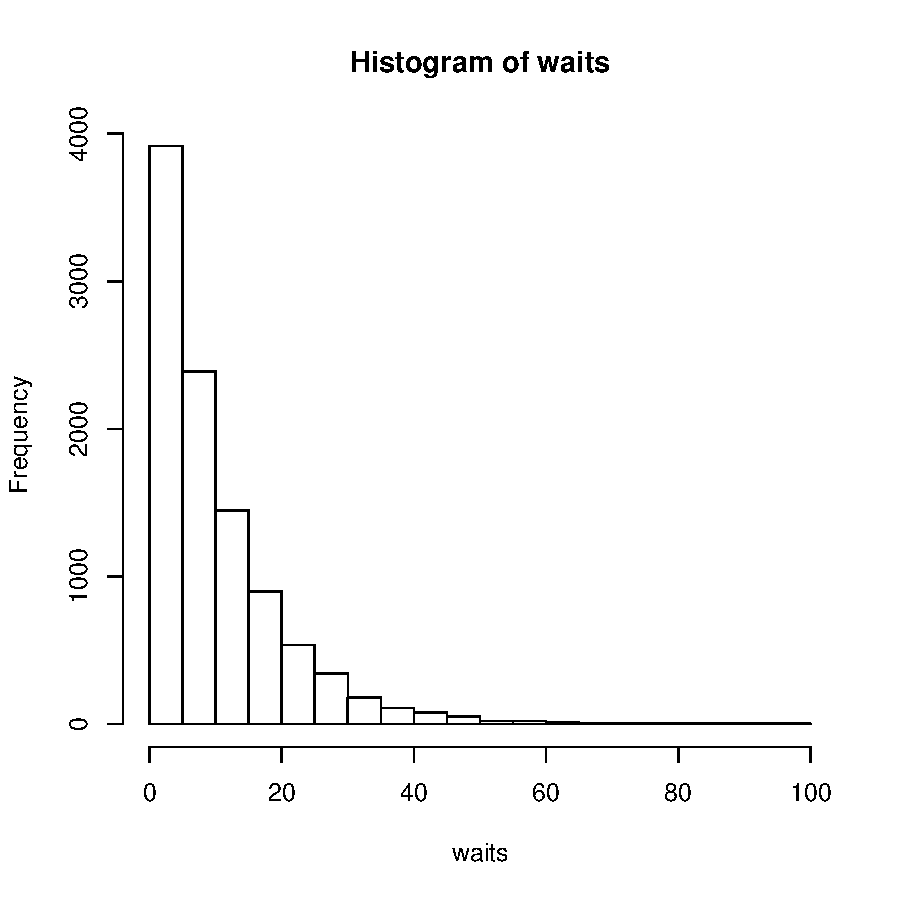
\includegraphics[width=4.0in]{HistDefault.pdf} 
% 
% The density seems to have a shape like that of the exponential
% parametric family.  (This is not surprising, because it {\it is}
% exponential, but remember we're pretending we don't know that.)
% 
% Here is the plot with 100 intervals:
% 
% 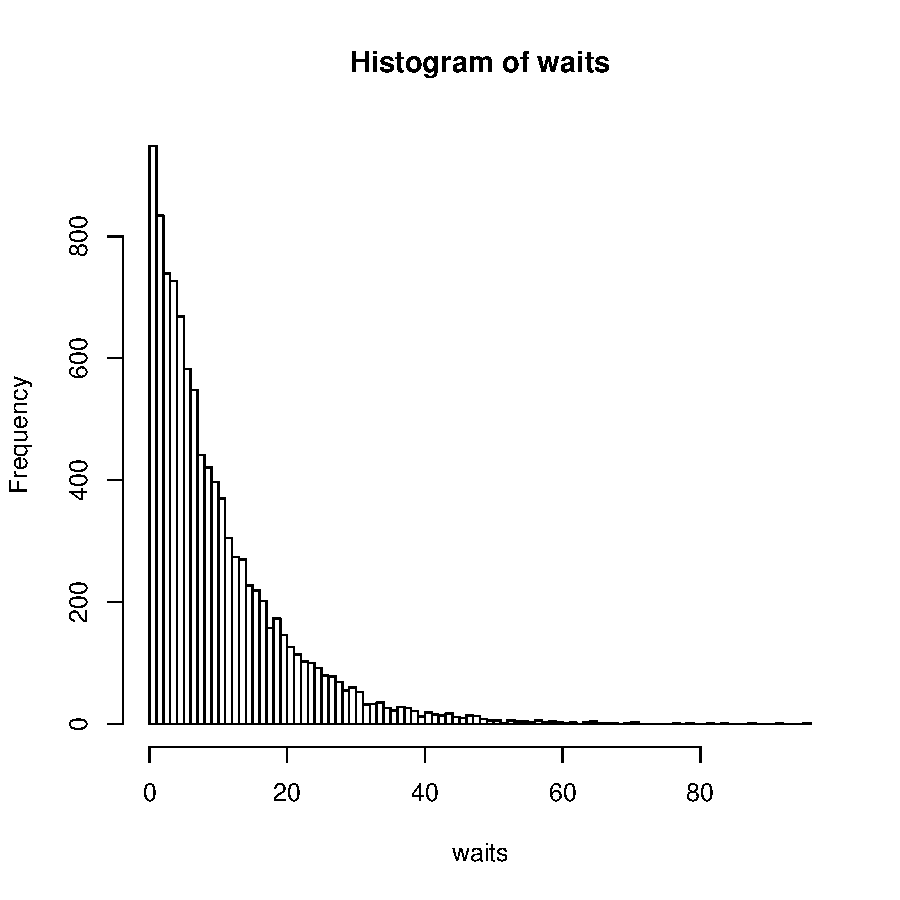
\includegraphics[width=4.0in]{Hist100.pdf} 
% 
% Again, a similar shape, though more raggedy.  

\section{Kernel-Based Density Estimation}

No matter what the interval width is, the histogram will consist of a
bunch of rectangles, rather than a curve.  We can get a smoother result
if we used more sophisticated methods, one of which is called {\bf
kernel-based} density estimation.  In base R, this is handled by the
function {\bf density()}.  

For any particular value of t, $\widehat{f_R(t)}$ above depends only on the
$R_i$ that fall into that interval.  If for instance some $R_i$ is just
barely outside the interval, it won't count.  We'll now change that.  

We need a set of weights, more precisely a weight function k, called the
{\bf kernel}.  Any nonnegative function which integrates to 1---i.e. a
density function in its own right---will work.  Our estimator is then

\begin{equation}
\label{kernel}
\widehat{f_R}(t) = \frac{1}{nh} \sum_{i=1}^{n} k \left ( \frac{t-R_i}{h} \right )
\end{equation}

To make this idea concrete, take k to be the uniform density on (-1,1),
which has the value 0.5 on (-1,1) and 0 elsewhere.  Then (\ref{kernel})
reduces to (\ref{prehisto}).  Note how the parameter h, called the {\bf
bandwidth}, continues to control how far away from to t we wish to go
for data points.

But as mentioned, what we really want is to include all data points, so
we typically use a kernel with support on all of $(-\infty, \infty)$.
In R's {\bf density()} function, the default kernel is that of the N(0,1) 
density.  

The bandwidth h controls how much smoothing we do; smaller values of h
place heavier weights on data points near t and much lighter weights on
the distant points.  

There is no surefire way to choose a good bandwidth.  A commonly used
rule of thumb is

\begin{equation}
h = 1.06 ~ s ~ n^{-1/5}
\end{equation}

where s is the sample standard deviation.

The default bandwidth in R is taken to the the standard
deviation of k.

% \checkpoint

\section{Example:  Baseball Player Data}

Some figures are plotted below for the baseball data, introduced in
Section \ref{baseball0}, for player weights, using functions in {\bf
ggplot2}:

\begin{itemize}

\item Figure \ref{b1} shows a histogram using the default number of
bins, 30, programmed as follows

\begin{lstlisting}
p <- ggplot(baseball)
p + geom_histogram(data=baseball,aes(x=Weight,y=..density..))
\end{lstlisting}

As conceded in the documentation for {\bf geom\_histogram()}, the
default tends to be not very good.  This was the case here, with a very
choppy figure.

\item I then tried a binwidth of 10 pounds, 

\begin{lstlisting}
p + geom_histogram(data=baseball,aes(x=Weight,y=..density..),binwidth=10)
\end{lstlisting}

This gave the much smoother plot in Figure \ref{b2}.

\item I then tried a kernel density estimate with the default bandwidth:

\begin{lstlisting}
p + geom_density(aes(x=Weight)) 
\end{lstlisting}

The result was similar to the histogram, but smoother, which is the
goal.  

\item Finally, I superimposed on that last plot a plot for the catchers
only (the latter in red):

\begin{lstlisting}
p + geom_density(aes(x=Weight)) + 
    geom_density(data=catch,aes(x=Weight,colour="red"))
\end{lstlisting}

As seen in Figure \ref{b4}, the catchers tend to be a bit heavier, and
have less variation than the players in general.

\end{itemize}

\begin{figure}[tb] 
\centerline{
\includegraphics[width=4.0in]{BaseballWtBWDefault.jpg} 
}
\caption{Histogram estimate, default binwidth}
\label{b1}  
\end{figure}

\begin{figure}[tb] 
\centerline{
\includegraphics[width=4.0in]{BaseballWtBW10.jpg} 
}
\caption{Histogram estimate, binwidth = 10}
\label{b2}  
\end{figure}

\begin{figure}[tb] 
\centerline{
\includegraphics[width=4.0in]{BaseballWtAll.jpg} 
}
\caption{Kernel estimate, all players, default bandwidth}
\label{b3}  

\end{figure}

\begin{figure}[tb] 
\centerline{
\includegraphics[width=4.0in]{BaseballWtAllPlusCatchers.jpg} 
}
\caption{Kernel estimate, all players plus catchers (red), default bandwidth}
\label{b4}  
\end{figure}

\section{More on Density Estimation in ggplot2}

See Section \ref{ggplot2dens}.

\section{Bias, Variance and Aliasing}

Nonparametric density estimation gives us an opportunity to apply the
principles of bias from Chapter \ref{chap:est}.

\subsection{Bias vs. Variance}

Recall from Section \ref{msesection} that for an estimator
$\widehat{\theta}$ of a population quantity $\theta$ we have that an
overall measure of the accuracy of the estimator is

\begin{equation}
\label{msehere}
E[(\widehat{\theta} - \theta)^2] = bias(\widehat{\theta})^2 +
Var(\widehat{\theta})
\end{equation}

In many cases there is a tradeoff between the bias and variance
components here.  We can have a smaller bias, for instance, but at the
expense of increased variance.  This is certainly the case with
nonparametric density estimation.

As an illustration, suppose the true population density is $f_R(t) = 4
t^3$ for t in (0,1), 0 elsewhere.  Let's use (\ref{prehisto}):

\begin{equation}
\widehat{f}_R(t) 
= \frac{\#(t-h,t+h))}{2hn}  
\label{prehisto1}
\end{equation}

What is the bias?  The numerator has a binomial distribution with n
trials and success probability\footnote{Note in the calculation here
that it doesn't matter whether we write $\leq t+h$ or $< t+h$, since R
is a continuous random variable.}

\begin{equation}
\label{usebinom}
p = P(t - h < R < t+h)
=  \int_{t-h}^{t+h} 4u^3 ~ du =
 (t+h)^4 - (t-h)^4
= 8t^3h+8th^3
\end{equation}

By the binomial property, the numerator of (\ref{prehisto1})  has
expected value np, and thus

\begin{equation}
E[\widehat{f_R}(t)] = 
\frac{np}{2nh} = 4t^3 + 4th^2
\end{equation}  

Subtracting $f_R(t)$, we have

\begin{equation}
\label{biasex}
bias[\widehat{f_R}(t)] = 4th^2
\end{equation}

So, the smaller we set h, the smaller the bias, consistent with
intuition.

How about the variance?  Again using the binomial property, the variance
of the numerator of (\ref{prehisto1}) is np(1-p), so that 

\begin{equation}
Var[[\widehat{f_R}(t)] = 
\frac{np(1-p)}{(2nh)^2} =
\frac{np}{2nh} \cdot \frac{1-p}{2nh} =
(4t^3+4th^2) \cdot \frac{1-p}{2nh} 
\end{equation}

This matches intuition too:  On the one hand, for fixed h, the larger n
is, the smaller the variance of our estimator---i.e. larger samples are
better, as expected.  On the other hand, the smaller we set h, the
larger the variance, because with small h there just won't be many $R_i$
falling into our interval (t-h,t+h).

So, you can really see the bias-variance tradeoff here, in terms of what
value we choose for h.\footnote{You might ask about finding the h to
minimize (\ref{msehere}).  This would not make sense in our present
context, in which we are simply assuming a known density in order to
explore the bias and variance issues here.  In practice, of course, we
don't know the density---that's why we are estimating it!  However,
some schemes (``plug-in'' methods) for selecting h find a rough estimate
of the density first, and then find the best h under the assumption that
that estimate is correct.}

\subsection{Aliasing}

There is another issue here to recognize:  The integration in
(\ref{usebinom}) tacitly assumed that $t-h > 0$ and $t+h < 1$.  But
suppose we are interested in $f_R(1)$.  Then the upper limit in the
integral in (\ref{usebinom}) will be 1, not t+h, which will
approximately reduce the value of the integral by a factor of 2.

This results in strong bias near the endpoints of the
support.\footnote{Recall that this term was defined in Section
\ref{continsupport}.}  Let's illustrate this with the same density
explored in our last section.

Using the general method in Section \ref{genrannumgen} for generating
random numbers from a specified distribution, we have that this
function will generate n random numbers from the density $4t^3$ on
(0,1):

\begin{lstlisting}
f <- function(n) runif(n)^0.25
\end{lstlisting}

So, let's generate some numbers and plot the density estimate:

\begin{lstlisting}
> plot(density(f(1000)))
\end{lstlisting}

The result is shown in Figure \ref{alias}.  Sure enough, the estimated
density drops after about t = 0.9, instead of continuing to rise.

\begin{figure}[tb] 
\centerline{
\includegraphics[width=3.0in]{Alias.jpg} 
}
\caption{Example of Aliasing}
\label{alias}  
\end{figure}

\section{Nearest-Neighbor Methods}

Consider (\ref{prehisto}) again.  We count data points that are
within a \underline{fixed distance} from t; the \underline{number} of
such points will be random.  With the nearest-neighbor approach, it's
just the opposite:  Now the \underline{number} will be fixed, while the
maximum \underline{distance} from t will be random.

Specifically, at any point t we find the k nearest $R_i$ to t, where k
is chosen by the analyst just like h is selected in the kernel case.
(And the method is are usually referred to as the {\it k-Nearest
Neighbor} method, kNN.)  The estimate is now

\begin{eqnarray}
\widehat{f}_R(t) &=& 
   \frac{k/n}{2\max_i |R_i - t|} \\ 
&=& 
   \frac{k}{2n \max_i |R_i - t|} \\ 
\end{eqnarray}


\section{Estimating a cdf}
\label{ecdfsec}

Let's introduce the notion of the {\bf empirical distribution function}
(ecdf), based on a sample $X_1,...,X_n$.  It is a sample estimate of a
cdf, defined to be the proportion of $X_i$ that are below t in the
sample.  Graphically, $\widehat{F}_X$ is a step function, with jumps at
the values of the $X_i$.

As a small example, say n = 4 and our data are 4.8, 1.2, 2.2 and
6.1.  We can plot the empirical cdf by calling R's {\bf ecdf()}
function:
 
\begin{Verbatim}[fontsize=\relsize{-2}]
> plot(ecdf(x))
\end{Verbatim}

The graph is in Figure \ref{ecdffig}.  (In {\bf ggplot2}, the function
{\bf stat\_ecdf()} is similar.)

\begin{figure}[tb] 
\centerline{
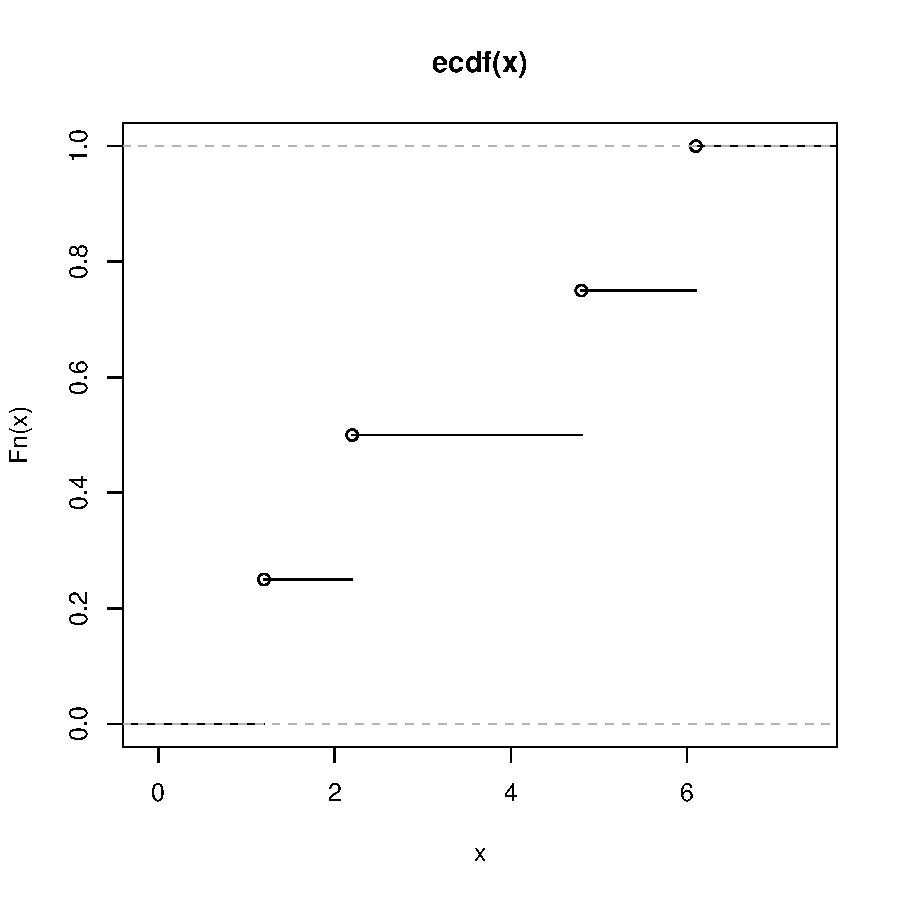
\includegraphics[width=3.0in]{EmpCDF.pdf} 
}
\caption{Empirical cdf, toy example}
\label{ecdffig}  
\end{figure}

\section{Hazard Function Estimation}

In principle, estimating a hazard function from data should be a direct
application of nonparametric density function methods.  In (\ref{hf}) we
would estimate the numerator with a kernel-based method, say, and the
cdf in the denominator using the ecdf (Section \ref{ecdfsec}).

However, the situation is complicated in that in many applications we
have {\bf censored data}, meaning that not all the data is available,
due to an event not yet happening.

Say we measure lifetimes of batteries, and that at the time we collect
our data, some of the batteries have died but some are still working.
The problem is that we don't know the lifetimes of the latter.  If one
has run, say, for 212 hours so far, we know that it's lifetime will be
at least 212, but we don't know the actual value yet.

This is an advanced topic, but a good starting point would be R's {\bf
muhaz} library in the CRAN repository.  See the references in the
documentation.

\section{For Further Reading}

To see an example of nonparametric density estimation applied to
biology, see this paper by a UCD professor:

Kernel Methods in Line and Point Transect Sampling. {\it Biometrics},
Mack, Y. P. and P. X. Quang (1998).  54, 609-619. 

Also see {\it All of Nonparametric Statistics}, Larry Wasserman 
Springer, 2007.

